\tikzstyle{majorStyle}=[shape = circle, minimum size = 6pt, inner sep = 2.2pt, draw]
\tikzstyle{major}=[shape = circle, minimum size = 6pt, inner sep = 2.2pt, draw]
\tikzstyle{minorStyle}=[shape = rectangle, minimum size = 6pt, inner sep = 2.2pt, draw]
\tikzstyle{minor}=[shape = rectangle, minimum size = 6pt, inner sep = 2.2pt, draw]
\tikzstyle{labeledStyle}=[shape = rectangle, minimum size = 6pt, inner sep = 2.2pt, draw]
\tikzstyle{VertexStyle} = []
\tikzstyle{EdgeStyle} = []
%\tikzstyle{unlabeledStyle}=[shape = circle, minimum size = 6pt, inner sep = 1.2pt, draw, fill]
\begin{figure}[htb]

\subfloat[]{\makebox[.5\textwidth]{
\begin{tikzpicture}[scale = 7]
\Vertex[style = major, x = 0.449999988079071, y = 0.949999999254942, L =
\tiny {$u$}]{v0}
\Vertex[style = minor, x = 0.150000005960464, y = 0.75, L = \tiny {$v_1$}]{v1}
\Vertex[style = minor, x = 0.349999994039536, y = 0.75, L = \tiny {$v_2$}]{v2}
\Vertex[style = major, x = 0.550000011920929, y = 0.75, L = \tiny {$v_3$}]{v3}
\Vertex[style = minor, x = 0.550000011920929, y = 0.550000011920929, L =
\tiny {$w$}]{v4}
\Edge[](v1)(v0)
\Edge[](v2)(v0)
\Edge[](v2)(v3)
\Edge[](v3)(v0)
\Edge[](v4)(v3)
\end{tikzpicture}
}}
%\subfloat[Figure 2]{\makebox[.5\textwidth]{
%\begin{tikzpicture}[scale = 7]
%\Vertex[style = major, x = 0.400, y = 0.900, L = \tiny {$u$}]{v0}
%\Vertex[style = minor, x = 0.150, y = 0.700, L = \tiny {$v_1$}]{v1}
%\Vertex[style = minor, x = 0.300, y = 0.700, L = \tiny {$v_2$}]{v2}
%\Vertex[style = major, x = 0.500, y = 0.700, L = \tiny {$v_3$}]{v3}
%\Vertex[style = major, x = 0.650, y = 0.700, L = \tiny {$v_4$}]{v4}
%\Vertex[style = minor, x = 0.650, y = 0.550, L = \tiny {$w$}]{v5}
%\Edge[](v1)(v0)
%\Edge[](v2)(v0)
%\Edge[](v2)(v3)
%\Edge[](v3)(v0)
%\Edge[](v4)(v0)
%\Edge[](v5)(v4)
%\end{tikzpicture}
%}}
\subfloat[]{\makebox[.5\textwidth]{
\begin{tikzpicture}[scale = 7]
\Vertex[style = major, x = 0.5, y = 0.849, L = \tiny {$u$}]{v0}
\Vertex[style = minor, x = 0.200, y = 0.650, L = \tiny {$v_1$}]{v1}
\Vertex[style = minor, x = 0.400, y = 0.650, L = \tiny {$v_2$}]{v2}
\Vertex[style = major, x = 0.600, y = 0.650, L = \tiny {$v_3$}]{v3}
\Vertex[style = major, x = 0.800, y = 0.650, L = \tiny {$v_4$}]{v4}
\Vertex[style = minor, x = 0.550, y = 0.449, L = \tiny {$w_1$}]{v6}
\Vertex[style = minor, x = 0.649, y = 0.449, L = \tiny {$w_2$}]{v5}
\Vertex[style = minor, x = 0.800, y = 0.449, L = \tiny {$w_3$}]{v7}
\Edge[](v1)(v0)
\Edge[](v2)(v0)
\Edge[](v3)(v0)
\Edge[](v4)(v0)
\Edge[](v5)(v3)
\Edge[](v6)(v3)
\Edge[](v7)(v4)
\end{tikzpicture}
}}

\subfloat[]{\makebox[.5\textwidth]{
\begin{tikzpicture}[scale = 7]
\Vertex[style = major, x = 0.500, y = 0.849, L = \tiny {$u$}]{v0}
\Vertex[style = minor, x = 0.400, y = 0.650, L = \tiny {$v_1$}]{v2}
\Vertex[style = minor, x = 0.500, y = 0.650, L = \tiny {$v_2$}]{v1}
\Vertex[style = major, x = 0.600, y = 0.650, L = \tiny {$v_3$}]{v3}
\Vertex[style = major, x = 0.800, y = 0.650, L = \tiny {$v_4$}]{v4}
\Vertex[style = minor, x = 0.500, y = 0.449, L = \tiny {$w_1$}]{v6}
\Vertex[style = minor, x = 0.699, y = 0.449, L = \tiny {$w_2$}]{v5}
\Edge[](v1)(v0)
\Edge[](v2)(v0)
\Edge[](v3)(v0)
\Edge[](v4)(v0)
\Edge[](v4)(v5)
\Edge[](v5)(v3)
\Edge[](v6)(v3)
\end{tikzpicture}
}}
\subfloat[]{\makebox[.5\textwidth]{
\begin{tikzpicture}[scale = 7,rotate=90]
\Vertex[style = minor, x = 0.349, y = 0.799, L = \tiny {$v_2$}]{v0}
\Vertex[style = minor, x = 0.649, y = 0.799, L = \tiny {$v_1$}]{v1}
\Vertex[style = major, x = 0.5, y = 0.650, L = \tiny {$u$}]{v2}
\Vertex[style = major, x = 0.5, y = 0.949, L = \tiny {$w_1$}]{v3}
\Vertex[style = major, x = 0.5, y = 0.5, L = \tiny {$v_3$}]{v4}
\Vertex[style = minor, x = 0.5, y = 0.350, L = \tiny {$w_2$}]{v5}
\Edge[](v2)(v0)
\Edge[](v2)(v1)
\Edge[](v3)(v0)
\Edge[](v3)(v1)
\Edge[](v4)(v2)
\Edge[](v5)(v4)
\end{tikzpicture}
}}
\caption{
Vertices drawn as circles have degree 4 in $G$ and vertices drawn as rectangles
have degree 3 in $G$.
}
\label{fig:hiltonzhao}
\end{figure}
